\documentclass[9pt,twocolumn,twoside]{pnas-new}

%% Some pieces required from the pandoc template
\providecommand{\tightlist}{%
  \setlength{\itemsep}{0pt}\setlength{\parskip}{0pt}}

% Use the lineno option to display guide line numbers if required.
% Note that the use of elements such as single-column equations
% may affect the guide line number alignment.

\usepackage[T1]{fontenc}
\usepackage[utf8]{inputenc}


\templatetype{pnasresearcharticle}  % Choose template

\title{From \emph{uh-oh} to \emph{tomorrow}: Predicting age of acquisition for
early words across languages}

\author[a,1]{Mika Braginsky}
\author[b]{Daniel Yurovsky}
\author[c]{Stephan Meylan}
\author[d]{Virginia Marchman}
\author[d]{Michael C. Frank}

  \affil[a]{Department of Brain and Cognitive Sciences, Massachusetts Insitute of
Technology, Cambridge, MA 02139}
  \affil[b]{Department of Psychology, University of Chicago, Chicago, IL 60637}
  \affil[c]{Department of Psychology, University of California Berkeley, Berkeley,
CA 94720}
  \affil[d]{Department of Psychology, Stanford University, Stanford, CA 94305}


% Please give the surname of the lead author for the running footer
\leadauthor{}

% Please add here a significance statement to explain the relevance of your work
\significancestatement{TODO}


\authorcontributions{Author contributions: TODO}

\authordeclaration{The authors declare no conflict of interest.}


\correspondingauthor{\textsuperscript{} }

% Keywords are not mandatory, but authors are strongly encouraged to provide them. If provided, please include two to five keywords, separated by the pipe symbol, e.g:
 \keywords{  TODO keywords   }

\begin{abstract}
Why do children learn some words earlier than others? Regularities and
differences in the acquisition patterns for words across languages yield
insights regarding the mechanisms guiding word learning. In a
large-scale corpus analysis, we use data from 38,212 children to
estimate the developmental trajectories of around 400 words in ten
languages, predicting them on the basis of independently-derived
linguistic, environmental, and conceptual factors. We examine the
consistency and variability of these predictors across languages, by
lexical category, and over development. By leveraging data at a
significantly larger scale than previous work, our analyses highlight
the power that emerges from unifying previously disparate theories, and
suggest areas of focus for further theory building.
\end{abstract}

\dates{This manuscript was compiled on \today}
\doi{\url{www.pnas.org/cgi/doi/10.1073/pnas.XXXXXXXXXX}}

\begin{document}

% Optional adjustment to line up main text (after abstract) of first page with line numbers, when using both lineno and twocolumn options.
% You should only change this length when you've finalised the article contents.
\verticaladjustment{-2pt}

\maketitle
\thispagestyle{firststyle}
\ifthenelse{\boolean{shortarticle}}{\ifthenelse{\boolean{singlecolumn}}{\abscontentformatted}{\abscontent}}{}

% If your first paragraph (i.e. with the \dropcap) contains a list environment (quote, quotation, theorem, definition, enumerate, itemize...), the line after the list may have some extra indentation. If this is the case, add \parshape=0 to the end of the list environment.

\acknow{TODO: acknowledgements}

Word learning is one of the central challenges of language acquisition.
Learners must integrate multiple information sources to map the word
forms they hear onto representations of their meanings. Across many
laboratory experiments and small-scale models, a number of strategies
have emerged as plausible components of word learning, including
tracking co-occurrence statistics between words and referents to deduce
word meaning across situations; attending to social cues like pointing
and eye gaze; relying on biases, such as a basic level category bias;
and drawing on knowledge of relations between words to use known
meanings to learn new ones.

Each of these strategies has been reliably demonstrated in the
constrained learning context of the laboratory, indicating that they are
possible parts of the word learning process. However, small-scale
experimental studies typically do not tell us whether these strategies
operate uniformly across children, ages, and languages. It is also
difficult to explore how strategies interact to create the longer-term
dynamics of vocabulary acquisition. How do the various strategies differ
in their relative contributions? And how does their influence change
over the course of development?

Our approach to addressing these questions is to use large-scale
vocabulary development data to examine these interactions. By
aggregating across a large number of children, we can look past
individual differences in acquisition to investigate not only which
words are relatively easy or hard to learn, but also what features
affect their acquisition. For example, distributional learning
strategies rely critically on frequency. Thus, to make a first
assessment of the contribution of distributional learning, we can
examine the relationship between the age at which words are typically
acquired and word frequency in child-directed speech.

Such an approach has revealed that in English, within a lexical
category, words that are more frequent in speech to children are likely
to be learned earlier (1). And further studies have found evidence for
semantic networks (2), neighborhood density (3), iconicity (4), and
linguistic distinctiveness (5) as additional predictors of age of
acquisition (AoA), suggesting that they are likely contributors to
vocabulary development. But these exciting findings are nevertheless
limited in their generality because they used different datasets,
focused on different predictors, and almost exclusively analyzed English
data. It is thus impossible to compare the relative importance of the
many relevant factors under consideration and to draw robust
conclusions.

To remedy this issue, we present analyses based on data from Wordbank
(\href{http://wordbank.stanford.edu}{wordbank.stanford.edu}), an open
repository of cross-linguistic language development data (6). By
aggregating administrations of the MacArthur-Bates Communicative
Development Inventory (7), a family of parent-report vocabulary
checklists, Wordbank provides large-scale vocabulary data based on
analogous instruments from almost 60,000 children in 17 different
language communities. Wordbank presents a novel resource for richer and
more powerful analyses of vocabulary learning over development and
across languages.

We integrate estimates of words' acquisition trajectories from Wordbank
with characterizations of the word learning environment from the CHILDES
database (8) and elsewhere, a multiple data source methodology
originated by (1). Building on this work, we examine interactions
between a variety of linguistic, environmental, and conceptual factors.
Using a similar approach on a high-density longitudinal corpus for a
single English-acquiring child, Roy et al. found that the length, usage
frequency, and mean length of the utterances in which it occurred were
all predictive of a word's AoA. But due to the nature of the dataset,
this analysis used production-based AoA estimates and was further
limited by relying on data from only one child acquiring a single
language.

Our work provides a complimentary analysis by using CDI comprehension
and production data available in Wordbank to look at the earliest words
that children learn across several different languages. We estimate
acqusition trajectories for approximately 400 words from CDIs in each of
10 languages. We also estimate each word's frequency and mean length of
utterance (MLU) based on the set of utterances in CHILDES containing the
word. Additionally, we obtain ratings of each word's concreteness,
valence, arousal, and relevance to babies from previously collected
norms. We use these measures to predict words' acquisition trajectories,
assessing the relative contributions of each, as well as how they change
over development and interact with lexical category. Each of these
analyses has the potential to advance our understanding of the
theoretical underpinnings of word learning.

A first theoretically-motivated question is which lexical categories are
most influenced by input-related factors, like frequency and utterance
length, compared with conceptual factors like concreteness and valence.
For example, the ``division of dominance'' theory suggests that nouns
might be more sensitive to cognitive factors, while predicates and
closed-class words might be more sensitive to linguistic factors (9). On
the other hand, on syntactic bootstrapping theories (10), nouns are
argued to be learned via frequent co-occurrence (operationalized by
frequency) while verbs might be more sensitive to syntactic factors
(operationalized here by utterance length), and neither would be
particularly sensitive to conceptual complexity (11).

A second question of interest is the extent to which there is
variability across languages in the relative importance of predictors.
For example, are there differences in the importance of grammar-related
factors in morphologically more complex languages like Russian and
Turkish, compared with simpler ones like English? Differences of this
type might be revealing of the degree to which learners face different
challenges in different language environments. Alternatively,
consistency may suggest the operation of similar learning mechanisms and
strategies that are not as dependent on the complexities of phonology,
morphology, and syntax in a particular language.

By incorporating a variety of theoretically-important factors, basing
our analysis on a large sample of words and children, and building
towards more cross-linguistic coverage, our study presents a more
thorough investigation of the question of what properties determine
words' learnability.

\section*{Data}\label{data}
\addcontentsline{toc}{section}{Data}

We use CDI data from Wordbank to estimate the acquisition trajectories
for words across 10 languages: Croatian, Danish, English, French
(Quebec), Italian, Norwegian, Russian, Spanish, Swedish, Turkish. We
then ask what factors are most important for predicting this trajectory.
Table \ref{table:lang_stats} gives an overview of our data sources.

\begin{table}[ht]
\centering
\begin{tabular}{lrr}
  \hline
Language & CDI Items & CDI Admins \\ 
  \hline
Croatian & 390 & 627 \\ 
  Danish & 383 & 6,112 \\ 
  English & 393 & 7,902 \\ 
  French (Quebec) & 396 & 1,364 \\ 
  Italian & 396 & 1,401 \\ 
  Norwegian & 381 & 12,225 \\ 
  Russian & 409 & 1,805 \\ 
  Spanish & 399 & 1,872 \\ 
  Swedish & 371 & 1,367 \\ 
  Turkish & 396 & 3,537 \\ 
   \hline
\end{tabular}
\caption{Dataset statistics} 
\label{table:lang_stats}
\end{table}

\subsection{Estimating Acquisition
Trajectory}\label{estimating-acquisition-trajectory}

To estimate the trajectory words' acquisition, we used vocabulary data
collected using the CDI, from both the Words \& Gestures (WG) form for
8-18 month olds and the the Words \& Sentences (WS) form for 16-36 month
olds. When filling out a CDI form, parents are asked to indicate whether
their child ``understands'' (comprehension) or ``understands and says''
(production) each of around 400-700 words (WG asks about both
comprehension and production, while WS asks only about production). From
these data, for each word on the CDI, we computed the proportion of
children at each age who were reported to understand/produce the word.
This results in a trajectory reflecting how commonly a word is learned
over age (see Table \ref{fig:demo_trajectories} for some examples). We
then predict on the basis of age, properties of the word, and the
interactions between age and each property.

\begin{figure*}

{\centering \includegraphics{journal_paper_files/figure-latex/demo_trajectories-1} 

}

\caption{Example trajectories for the words "dog" and "jump" across language.}\label{fig:demo_trajectories}
\end{figure*}

\begin{table}[b!]
\centering
\begin{tabular}{lll}
  \hline
Predictor & Highest & Lowest \\ 
  \hline
frequency & you, it, that & cockadoodledoo, grrr, church \\ 
  MLU & when (question), day, store & peekaboo, ouch, hello \\ 
  final\_frequency & book, it, there & give, when (question), put \\ 
  solo\_frequency & no, yes, what & tooth, feed, aunt \\ 
  length & cockadoodledoo, refrigerator,
 rocking chair & i, go, hi \\ 
  concreteness & apple, baby, ball & how, now, that \\ 
  valence & happy, hug, love & sick, hurt (description), ouch \\ 
  arousal & naughty, money, scared & shh, asleep, blanket \\ 
  babiness & baby, bib, bottle & donkey, penny, jeans \\ 
   \hline
\end{tabular}
\caption{Words with the lowest and highest values for each predictor in English.} 
\label{table:extremes}
\end{table}

\begin{figure*}

{\centering \includegraphics{journal_paper_files/figure-latex/lang_coefs-1} 

}

\caption{TODO}\label{fig:lang_coefs}
\end{figure*}

\begin{figure*}

{\centering 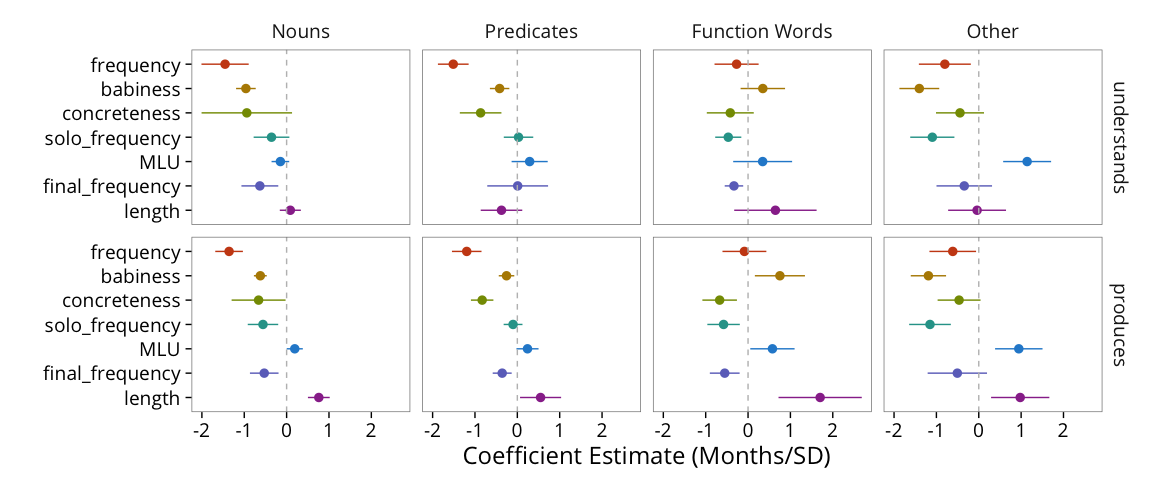
\includegraphics{journal_paper_files/figure-latex/lexcat_coefs-1} 

}

\caption{TODO}\label{fig:lexcat_coefs}
\end{figure*}

\section*{Predictors}\label{predictors}
\addcontentsline{toc}{section}{Predictors}

Each of our predictors is derived from independent sources. For each
word that appears on the CDI forms in each of our 10 languages, we
obtained an estimate of its frequency in child-directed speech, the mean
length of utterances in which it appears in child-directed speech, its
length in characters, and ratings of its concreteness, valence, arousal,
and relevance to babies. Items such as \emph{child's own name} were
excluded. Example words for these predictors in English are shown in
Table \ref{table:extremes}.

Frequency and MLU are measured relative to the word's language. But
since existing datasets for conceptual ratings are primarily available
for English, we mapped all words onto translation equivalents across CDI
forms, allowing us to use the ratings for English words across
languages. While necessarily imperfect, this method allows us to examine
languages for which limited resources exist. Translation equivalents are
available in the Wordbank database using the \texttt{wordbankr} package
in \texttt{R} (6).

Each numeric predictor was centered and scaled so that all predictors
would have comparable units. Lexical category was determined on the
basis of the conceptual categories presented on the CDI form (e.g.,
``Animals''), such that the Nouns category contains common nouns,
Predicates contains verbs and adjectives, Function Words contains
closed-class words, and Other contains the remaining items (12).

\subsection{Frequency}\label{frequency}

For each language, we estimated word frequency from unigram counts based
on all corpora in CHILDES for that language. Each word's count includes
the counts of words that share the same stem (so that \emph{dogs} counts
as \emph{dog}) or are synonymous (so that \emph{father} counts as
\emph{daddy}). For polysemous word pairs (e.g., \emph{orange} as in
color or fruit), occurrences of the word in the corpus were split
uniformly between the senses on the CDI. Counts were normalized to the
length of each corpus and then log transformed.

\subsection{Solo and Final
Frequencies}\label{solo-and-final-frequencies}

Using the same dataset as for frequency, we estimated the frequency with
which each of word occurs as the sole word in an utterance, and the
frequency with which it appears as the final word of an utterance (not
counting single-word utterances). Since both of these estimates are by
necessity highly correlated with frequency, we residualized unigram
frequency out of both of them, so that values reflect an estimate of the
effect of solo/final frequency over and above frequency itself.

\subsection{MLU}\label{mlu}

For each language, we estimated each word's MLU by calculating the mean
length in words of the utterances in which that word appeared, for all
corpora in CHILDES for that language. Words that only occurred in one
utterance were excluded.

\subsection{Length}\label{length}

We computed the number of characters in each word in each language.
While imperfect, this metric of length is highly correlated with number
of phonemes and syllables (13).

\subsection{Concreteness}\label{concreteness}

We used previously collected norms for concreteness (14), which were
gathered by asking adult participants to rate how concrete the meaning
of each word is on a 5-point scale from abstract to concrete. For the
{[}TODO{]} CDI words that were not part of the collected norms, we
imputed ratings from the mean of all CDI words' ratings.

\subsection{Valence and Arousal}\label{valence-and-arousal}

We also used previously collected norms for valence and arousal (15),
for which adult participants were asked to rate words on a 1-9
happy-unhappy scale (valence) and 1-9 excited-calm scale (arousal). For
the TODO CDI words that were not part of the collected norms (mostly
function words), we imputed ratings from the mean of all CDI words'
ratings.

\subsection{Babiness}\label{babiness}

Lastly, we used previously collected norms of ``babiness'', a measure of
association with infancy (4) for which adult participants were asked to
judge a word's relevance to babies.

\section*{Analysis}\label{analysis}
\addcontentsline{toc}{section}{Analysis}

For all analyses, we use logistic regression mixed-effects models to
predict the numbers of children who understand/produce each word at each
age from age, the above predictors, and the interactions of age with the
predictors. We present three analyses of these models: 1) the relative
values of predictors for different languages and measures; 2) their
interactions with age; and 3) their breakdown by lexical category.

\subsection{Main Effects}\label{main-effects}

Figure \ref{fig:lang_coefs} shows the coefficient estimate for each
predictor in each language. We find that babiness, frequency, MLU, and
concreteness are relatively stronger predictors of age of acquisition
across languages. Given the emphasis on frequency effects in the
language acquisition literature (16), one might have expected frequency
to dominate, but several other predictors are just as strong in this
analysis. Some factors previously argued to be important for word
learning, namely valence and arousal, appear to have limited relevance
when compared to other factors.

A potential concern for comparing these coefficient estimates is
predictor collinearity. Fortunately, in every language, the only high
correlations were between frequency and number of characters, a
reflection of Zipf's Law (17), and between frequency and concreteness,
probably as a consequence of the complexity bias (13).

Overall, there is considerable consistency in how the predictors pattern
in various languages -- a priori, it could have been the case that
different languages have wildly different effects of experiential
vs.~structural factors, but this is not what we seem to find. Another
observation of note is the differences between coefficient estimates
between measures: the largest asymmetry is displayed by length, which is
far more predictive for production than comprehension. Thus as measured
here, length seems to be playing more the role of how difficult a word
is to say than how difficult it is to remember.

\subsection{Age Interactions}\label{age-interactions}

Next, we wanted to examine not just the contributions of various factors
to word learning, but also how their relative importance changes over
development. Across languages, positive age interactions can be seen for
concreteness and frequency (i.e.~their effects increase with age).
Conversely, there are negative age interactions for babiness and valence
in comprehension and for solo frequency in production.

\subsection{Lexical Category}\label{lexical-category}

Previous work gives reason to believe that predictors' relationship with
age of acquisition differs among various lexical categories (1). To
investigate these effects, we separated our data by lexical category and
fit separate models for each category. Figure \ref{fig:lexcat_coefs}
shows the resulting coefficient estimates. Frequency matters most for
nouns and comparatively little for function words, while MLU is
irrelevant for both nouns and predicates, but is highly informative for
function words.

\section*{Discussion}\label{discussion}
\addcontentsline{toc}{section}{Discussion}

What makes words easier or harder for young children to learn? Previous
experimental work has largely addressed this question using small-scale
experiments. While such experiments can identify sources of variation,
they typically do not allow for different sources to be compared in
detail. In contrast, observational studies allow the effects of
individual factors (with frequency being the most common) to be measured
across ages and lexical categories (1). Scale comes at a cost in terms
of detail, however, since the availability of both predictors and
outcome data has been quite limited.

By including 10 languages and 9 predictors, our current work expands the
scope of previous observational studies of age of acquisition. Our data
show a number of patterns that confirm and expand previous reports.
First, predictors changed in relative importance across development. For
example, certain concepts that were more strongly associated with babies
appeared to be learned early for children across languages (18).

Second, we found general consistency in predictor coefficients across
languages (even as overall model fit varied, at least in part due to the
amount and quality of data for different languages). This consistency
supports the idea that differences in culture or language structure do
not lead to fundamentally different acquisition strategies, at least at
the level of detail we were able to examine.

Lastly, the predictors varied in strength across lexical categories.
Frequent, concrete nouns were learned earlier, consistent with theories
that emphasize the importance of early referential speech (19). But for
predicates, concreteness was somewhat less important, and for function
words, MLU was most predictive. Overall these findings are consistent
with theories that emphasize the role of linguistic structure over
conceptual complexity in the acquisition of other lexical categories
beyond nouns (9, 11).

Despite its larger scope, our work shares a number of important
limitations with previous studies. First and foremost, our approach is
to predict one set of individuals with data about the experience of a
completely different set and ratings of concepts gathered from yet
others. In contrast to dense-data analyses (5), this approach
fundamentally limits the amount of variability we will be able to
capture. In addition, the granularity of the predictors that can be
extracted from corpus data and applied to every word is necessarily
quite coarse. Ideally, predictors could be targeted more specifically at
particular theoretical constructs of interest (for example, the patterns
of use for specific predicates).

{[}TODO: end on a high note?{]}

\subsection*{Supporting Information
(SI)}\label{supporting-information-si}
\addcontentsline{toc}{subsection}{Supporting Information (SI)}

TODO

\showmatmethods
\showacknow
\pnasbreak

\hypertarget{refs}{}
\hypertarget{ref-goodman2008}{}
1. Goodman JC, Dale PS, Li P (2008) Does frequency count? Parental input
and the acquisition of vocabulary. \emph{Journal of child language}
35(3):515.

\hypertarget{ref-hills2009}{}
2. Hills TT, Maouene M, Maouene J, Sheya A, Smith L (2009) Longitudinal
analysis of early semantic networks: Preferential attachment or
preferential acquisition? \emph{Psychological Science} 20(6):729--739.

\hypertarget{ref-stokes2010}{}
3. Stokes SF (2010) Neighborhood density and word frequency predict
vocabulary size in toddlers. \emph{Journal of Speech, Language, and
Hearing Research} 53(3):670--683.

\hypertarget{ref-perry2015}{}
4. Perry LK, Perlman M, Lupyan G (2015) Iconicity in English and Spanish
and its relation to lexical category and age of acquisition. \emph{PloS
one} 10(9):e0137147.

\hypertarget{ref-roy2015}{}
5. Roy BC, Frank MC, DeCamp P, Miller M, Roy D (2015) Predicting the
birth of a spoken word. \emph{Proceedings of the National Academy of
Sciences} 112(41):12663--12668.

\hypertarget{ref-frank2016}{}
6. Frank MC, Braginsky M, Yurovsky D, Marchman VA (2016) Wordbank: An
open repository for developmental vocabulary data. \emph{Journal of
Child Language}.

\hypertarget{ref-fenson2007}{}
7. Fenson L (2007) \emph{MacArthur-Bates Communicative Development
Inventories: User's guide and technical manual} (Paul H. Brookes
Publishing Company).

\hypertarget{ref-macwhinney2000}{}
8. MacWhinney B (2000) \emph{The CHILDES project: The database}
(Psychology Press).

\hypertarget{ref-gentner2001}{}
9. Gentner D, Boroditsky L (2001) Individuation, relativity, and early
word learning. \emph{Language Acquisition and Conceptual Development}
(Cambridge University Press).

\hypertarget{ref-gleitman1990}{}
10. Gleitman L (1990) The structural sources of verb meanings.
\emph{Language acquisition} 1(1):3--55.

\hypertarget{ref-snedeker2007}{}
11. Snedeker J, Geren J, Shafto CL (2007) Starting over: International
adoption as a natural experiment in language development.
\emph{Psychological science} 18(1):79--87.

\hypertarget{ref-bates1994}{}
12. Bates E, et al. (1994) Developmental and stylistic variation in the
composition of early vocabulary. \emph{Journal of Child Language}
21(01):85--123.

\hypertarget{ref-lewisunderreview}{}
13. Lewis ML, Frank MC (under review) The length of words reflects their
conceptual complexity.

\hypertarget{ref-brysbaert2014}{}
14. Brysbaert M, Warriner AB, Kuperman V (2014) Concreteness ratings for
40 thousand generally known English word lemmas. \emph{Behavior research
methods} 46(3):904--911.

\hypertarget{ref-warriner2013}{}
15. Warriner AB, Kuperman V, Brysbaert M (2013) Norms of valence,
arousal, and dominance for 13,915 English lemmas. \emph{Behavior
research methods} 45(4):1191--1207.

\hypertarget{ref-ambridge2015}{}
16. Ambridge B, Kidd E, Rowland CF, Theakston AL (2015) The ubiquity of
frequency effects in first language acquisition. \emph{Journal of child
language} 42(02):239--273.

\hypertarget{ref-zipf1935}{}
17. Zipf GK (1935) The psycho-biology of language.

\hypertarget{ref-tardif2008}{}
18. Tardif T, et al. (2008) Baby's first 10 words. \emph{Developmental
Psychology} 44(4):929.

\hypertarget{ref-baldwin1995}{}
19. Baldwin DA (1995) Understanding the link between joint attention and
language. \emph{Joint attention: Its origins and role in
development}:131--158.



% Bibliography
% \bibliography{pnas-sample}

\end{document}

